\chapter{Measuring mass using Gravitational Lensing}

\begin{quote}
	``The observation of such a gravitational lens effect promises to
		furnish us with the simplest and most accurate determination of
		nebular [sic] masses. No thorough search for these effects has
		yet been undertaken."  --- Fritz Zwicky, 1937
\end{quote}

\section{Introduction}

Gravitational lensing is the bending of the paths of photons in the
distortion of space-time caused by mass (i.e., by gravity). Gravitational
lensing manifests in the universe on a range of mass and length
scales. At the smallest scales --- the Solar System --- the mass of the
Sun can cause an subtle shift in the apparent positions of background
stars along lines of sight close to the Sun. This effect, only visible
during an eclipse (otherwise the light from the Sun precludes observing
the background stars) was first observed by Sir Arthur Eddington in
1919, and provided crucial early support to Einstein's theory of General Relativity, because the
observed effect agreed with his predictions.

In the 1930s the astronomer Fritz Zwicky showed that galaxies (then
still referred to as nebulae, as you can see in the quote above) and
clusters of galaxies might be $the$ best place in the universe to
search for gravitational lensing, and argued that observation of this
effect would be the best and cleanest way to measure the mass of these
objects. 

In this lab, you will find examples of gravitational lenses on cosmological scales,
using data from the 
%Sloan Digital Sky Survey (SDSS)
Hubble Legacy Archive (HLA) database.
%, visualized in Google Sky.
Then you will use the image of a distant
object created by the galaxy lens to find the mass of the galaxy or
galaxy cluster that is acting as the lens.

\section{Gravitational lensing theory}

The basics of gravitational lensing can be understood from a simple
diagram shown in Figure~\ref{gl:fig:geometry}, coupled with the knowledge that mass bends the paths of
photons. Consider an observer, O, a lensing mass, L, and a source
of photons, S. We will consider the cosmological scale case here, so S
might be a distant galaxy or quasar, and L a cluster of
galaxies or a lone massive galaxy, situated between O and S. 

\begin{figure}
	\begin{center}
		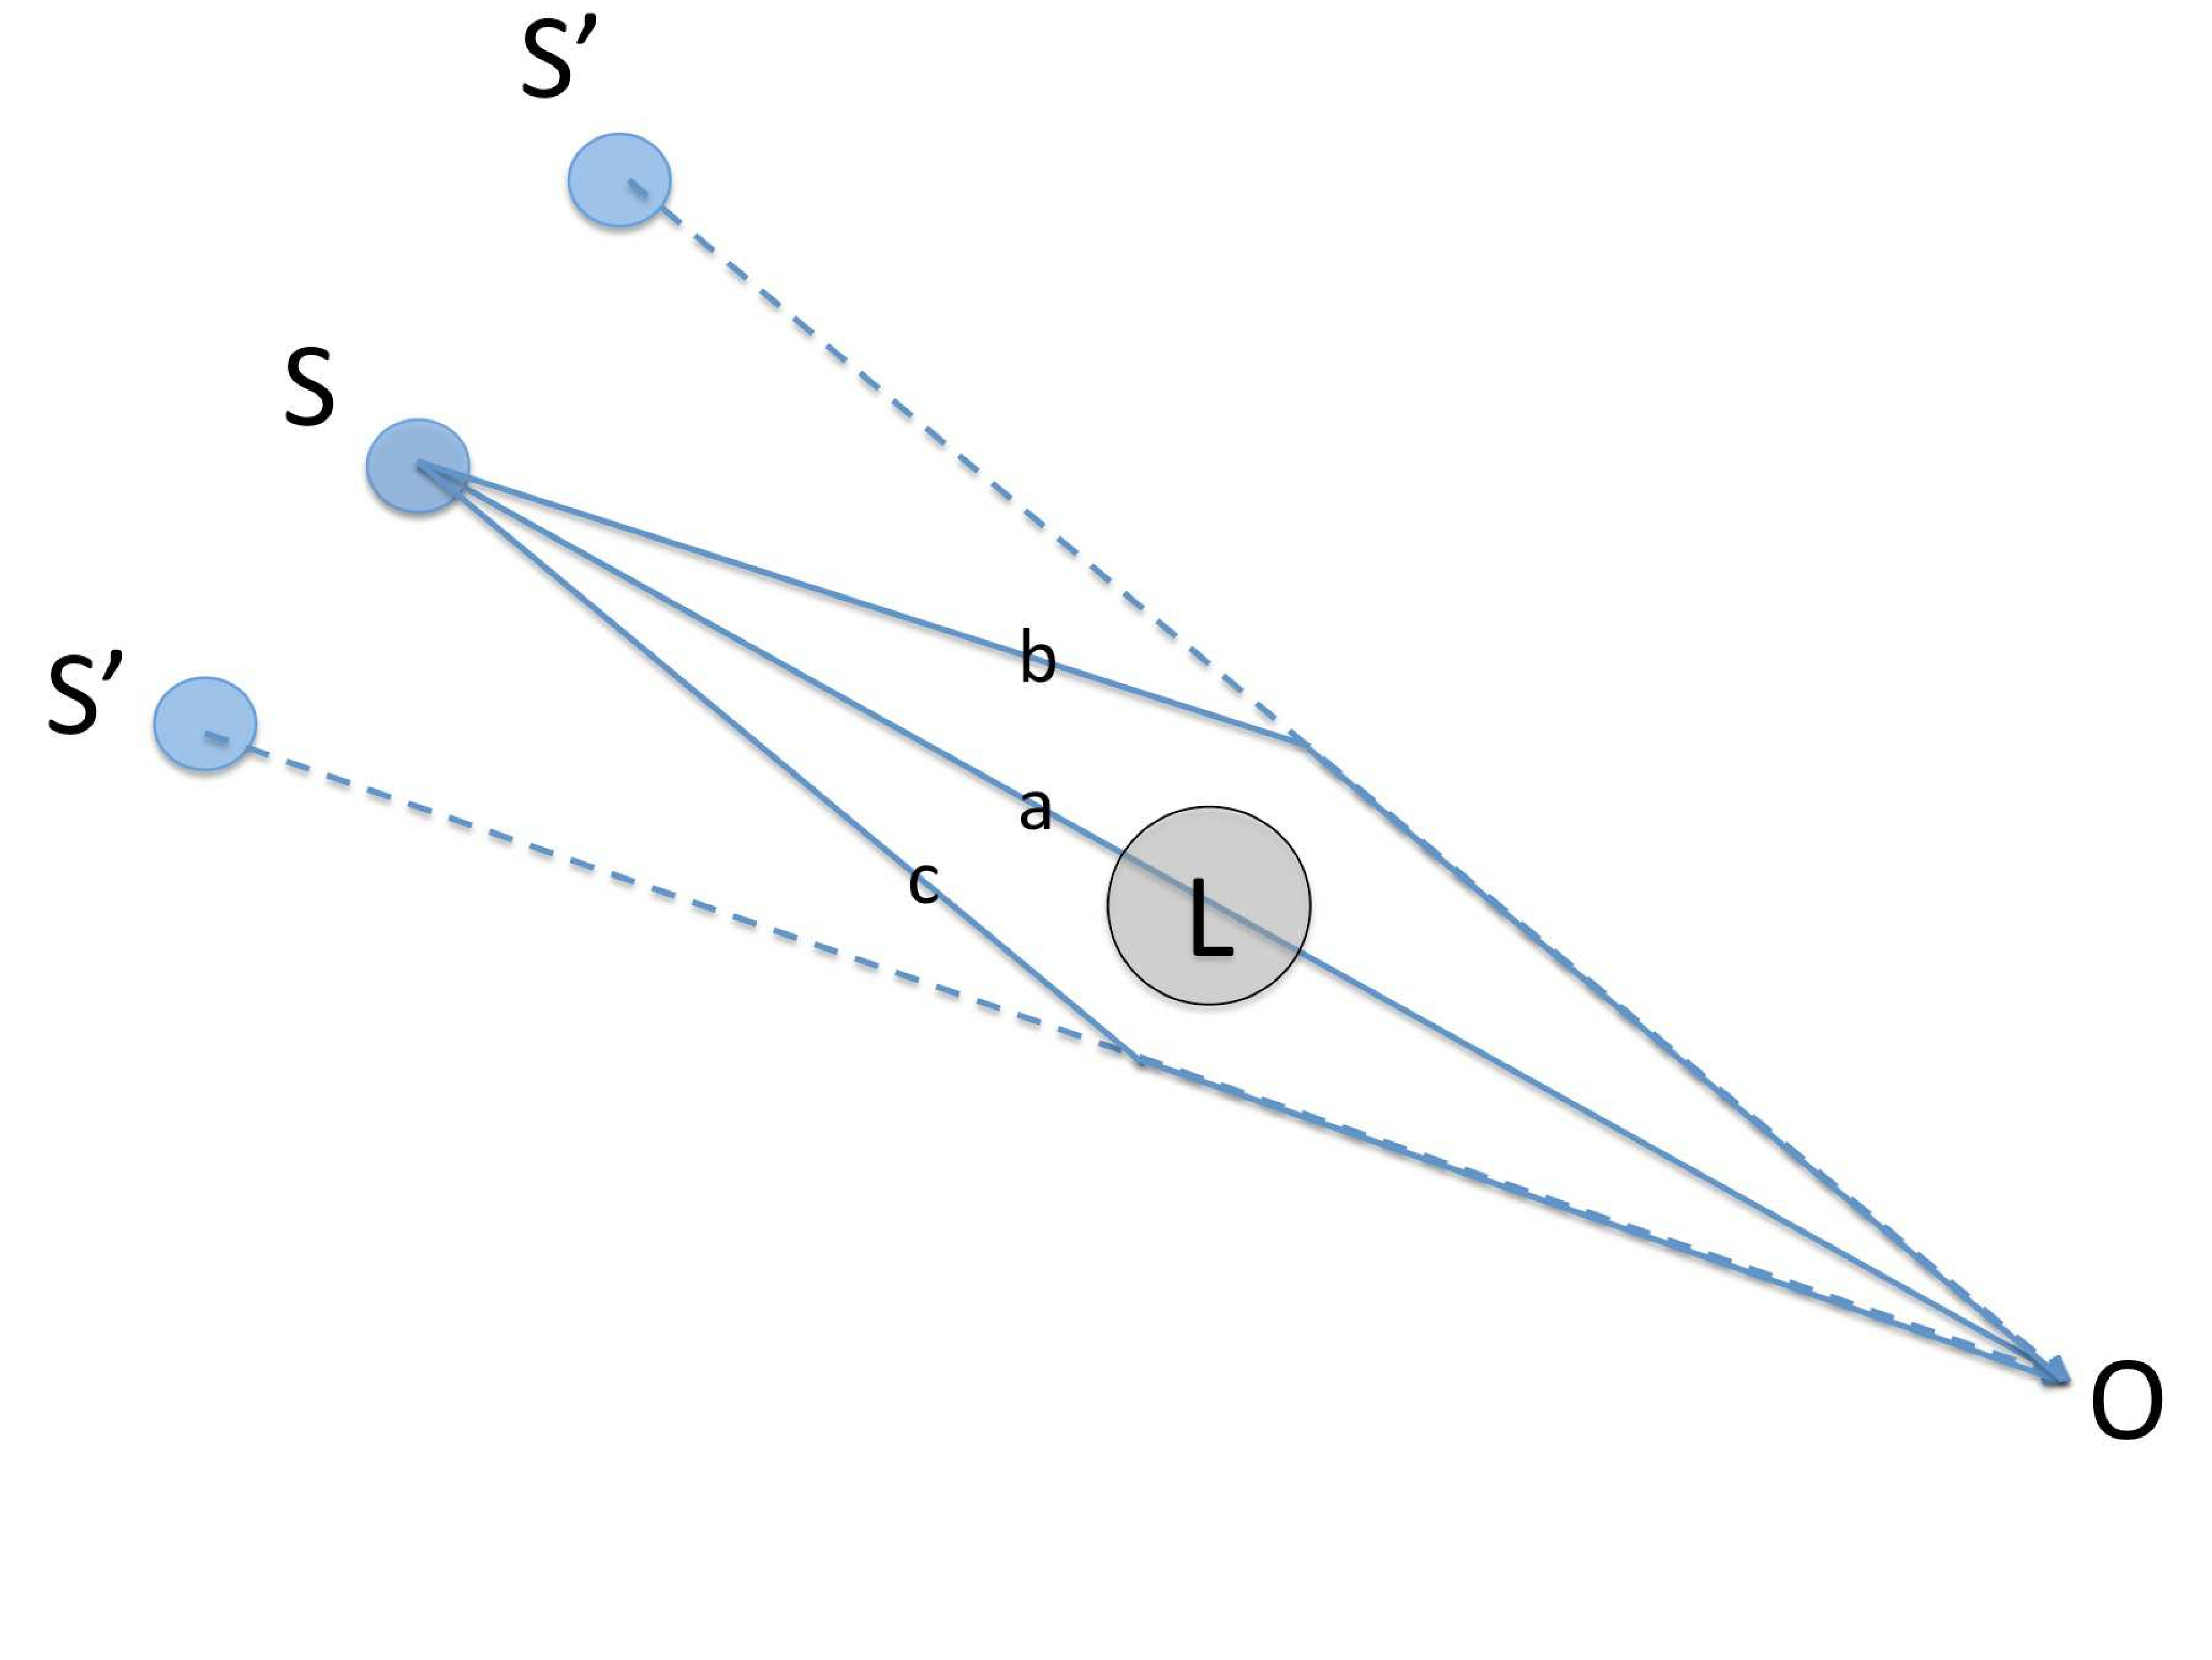
\includegraphics[scale=0.20]{gravitational-lensing/lensing1}
	\end{center}
	\caption{Diagram showing the geometry of source (S), observer (O), and gravitational lens (L). The source that would appear along direction OS without the lens, in the presence of lens appears along directions S$^{\prime}$ instead.}\label{gl:fig:geometry}
\end{figure}

Photons are being emitted by S in all directions, and normally in the
absence of an intervening lens, O will see the source at a position
corresponding to the direction from which photons are arriving from
the source (case a). With an intervening lens L in place, other
photons which normally would not arrive at O have their paths diverted
as they pass by L, and end up being observed by O (cases b,c). Under
this circumstance the observer 'sees' images of S not at its actual
location but at virtual locations corresponding to the direction from
which the diverted photons are arriving (images S').  If the alignment
between S, L and O is perfectly along a line, and L is circularly
symmetric on the sky, then the image S' is a ring on the sky. This is
called an Einstein Ring -- a sketch of this from the observer's
perspective, and actual examples from Hubble Space Telescope
observations of lensing systems found in the Sloan Digital Sky survey (SDSS) are shown in Figure~\ref{gl:fig:rings}.

\begin{figure}
	\centering
	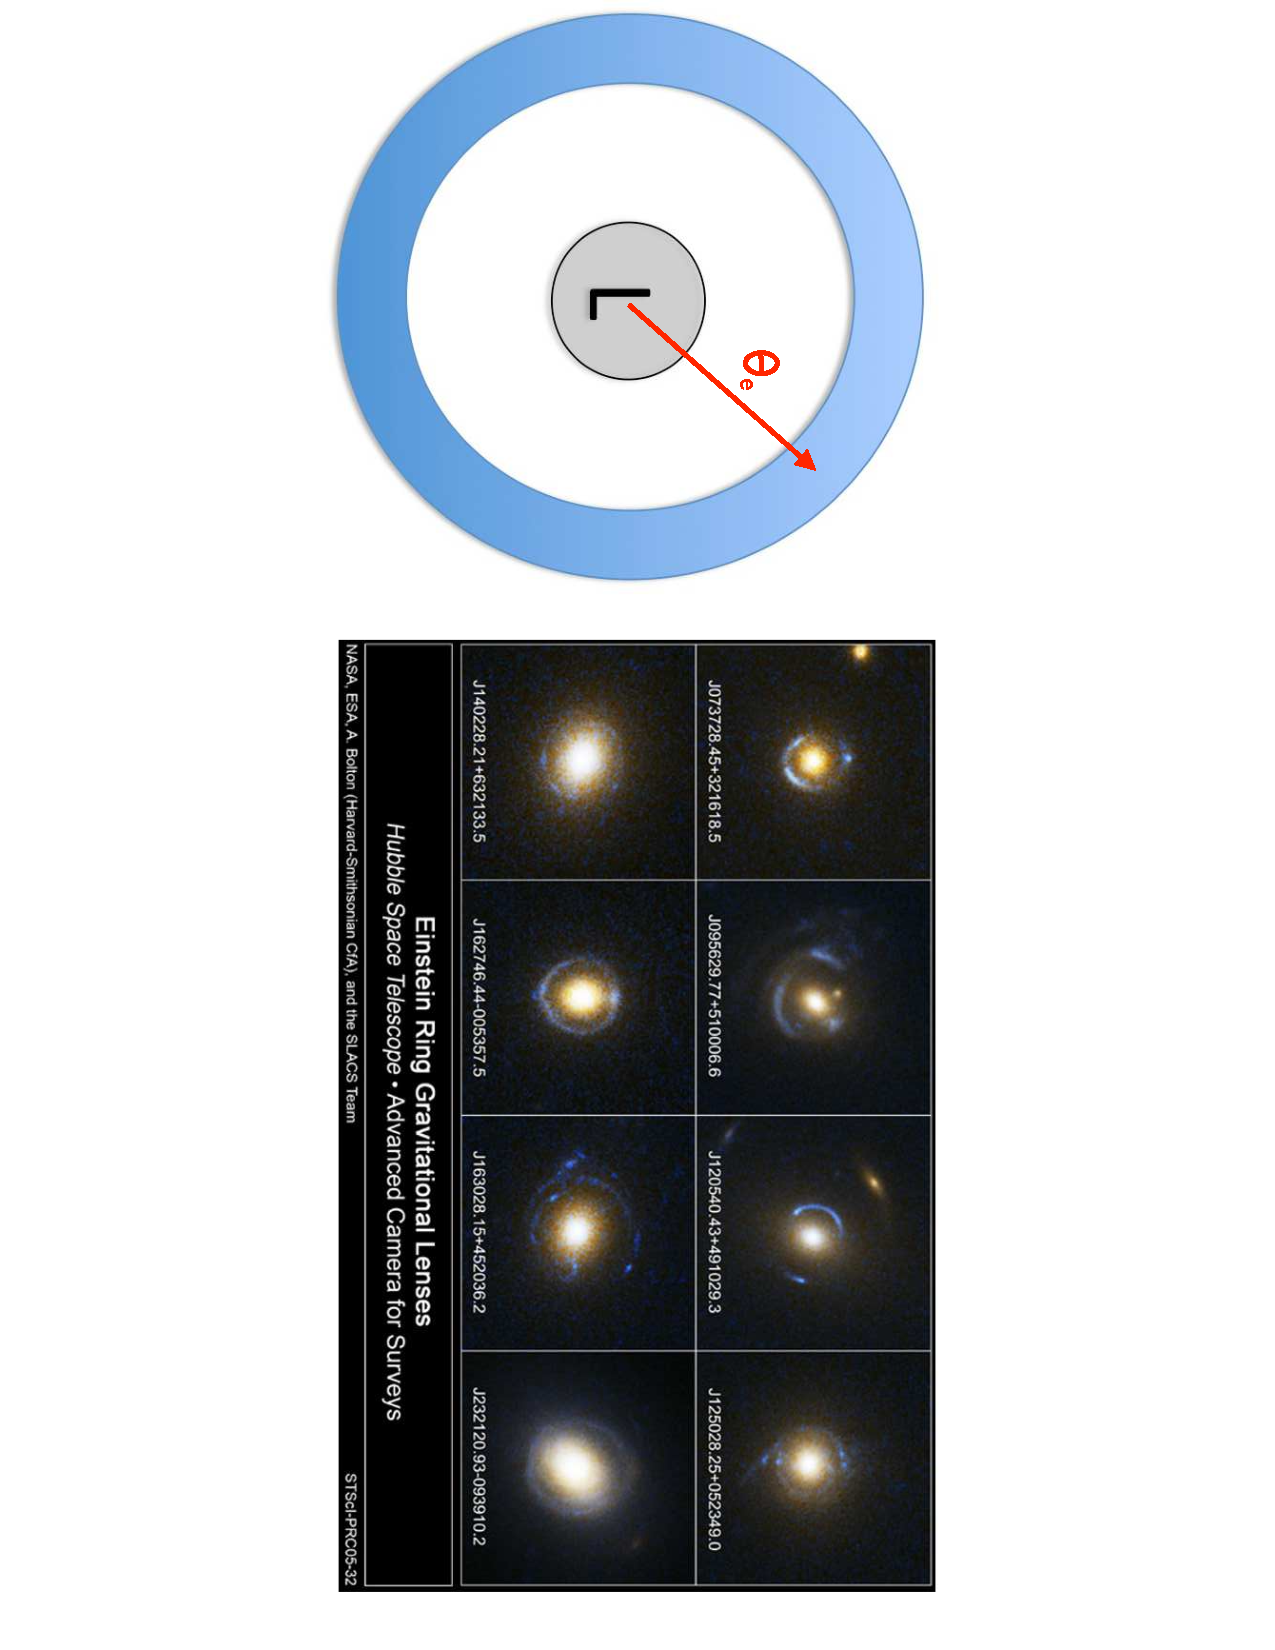
\includegraphics[width=0.9\textwidth, angle=90]{gravitational-lensing/lensing2a}
	\caption{A sketch of the Einstein ring from the observer's perspective
		(left), and actual examples from Hubble Space Telescope observations
		of lensing systems found in the SDSS (right). The distance from the
		center of the ring to the ring itself is called \textit{the Einstein
			radius} noted as $\theta_e$ in the sketch above, and in the equations below. It is this quantity which you will be estimating from the images, once you have identified several systems showing strong lensing.}\label{gl:fig:rings}
\end{figure}

Note that the degree to which the photon's path is deviated is
proportional to the mass of L, with a larger mass providing a greater
deflection. {\emph The apparent radius of the Einstein ring on the sky thus
	provides a measure of the mass of the lens interior to the ring.} The
size of the ring is also related to the distance along the line of
sight between S, L and O; to robustly determine the mass of the lens
we must also know these distances. 

Also note that the alignment between S, L and O is rarely perfect, and
the lens L is rarely perfectly circular on the sky; the result of this
is that complete Einstein rings are very rare and most lensed images
S' are arcs which look like portions of a ring image. 

\subsection*{Lab Tasks}

\begin{steps}
%	\item Your TA will provide a conical lens that acts as an optics analog of
%	the gravitational lens effect. Use this and the grid of points on the
%	last page of the lab manual to explore the lensing effect visually; include a
%	few sketches of lensed points in your lab report.
	\item To visualize how the lensing works, watch the animation at the following link:
\begin{framed} \url{https://public.nrao.edu/gallery/animation-of-a-gravitational-lens-creating-an-einstein-ring/}
\end{framed}
	Note that real lenses move much more slowly and are actually stationary on the human timescale, and that only
	precise alignment yields full rings and that partial arcs are much
	more typical.
	
	\item Take a few minutes to explore some images of
	gravitational lensing recorded by instruments on the Hubble Space
	Telescope. An extensive gallery of images can be found at \url{http://hubblesite.org/images/news/18-gravitational-lensing}
	
\end{steps}

The type of lensing we are exploring in this lab is called strong
lensing, and is the most obvious manifestation of the bending of
photon paths by gravity. Other types of lensing have also been observed.

When the lens involved has the mass of a star (apart from the specific
case of the Sun, discussed above) rather than a galaxy or cluster of
galaxies, then the radius of the Einstein ring is typically
micro-arcseconds. In that case the lensing cannot be observed as a
spatial distortion directly in the image (no telescope produces
images with a resolution fine enough to see micro-arcsecond
structures) however the focusing effect of lensing still produces an
enhancement in brightness which can be observed. This type of lensing
is often referred to as micro lensing.

A further manifestation of lensing is the weak distortion of the
images of background objects which are well away from the observer to
lens line-of-sight. In that case the background source is not imaged
into a ring or arc or multiple images, but there is still a discernible pattern of
distortion around the massive object. This pattern can be
analyzed statistically, and provides another mass estimate for the
lens. This effect, not surprisingly, is known as weak lensing.
%You can see this effect for yourself; when using the plastic conical optic, note the effect of the lens on the grid of points away from the central peak, as this looks very much like weak lensing in the real universe.

Gravitational lensing as a phenomenon has a wide range of
manifestations in the universe, and it is now an important technique
for study mass in the universe on a range of scales, from extrasolar
planets through to the largest structures. What began as a theoretical
curiosity in the early 20th century is now one of the most powerful
tools that we have to learn more about the cosmos. In the remainder of
this lab you'll find a few astronomical lenses to work with and then apply some of
the basics of strong lensing to measures the masses of galaxies and
clusters of galaxies.


%\section*{Finding a Few Strong Lenses}
%
%The SDSS has been a bonanza for the study of strong gravitational
%lenses, as it has allowed for the discovery of several hundred lenses
%at both galaxy and cluster of galaxy scales, for the first time. The
%first gravitational lens was discovered only in 1979 --- 42 years after
%Zwicky predicted that one should look for this effect near galaxies ---
%and until the SDSS only handfuls of these systems were known in the
%entire universe.  
%
%After SDSS found them, the Hubble Space Telescope took detailed images of them.
%
%In this section of the lab, you will search for several gravitational lenses using their names.
%
%%In this section of the lab you will look through a
%%list of locations in the SDSS -- looking at both individual galaxies
%%and cluster of galaxies -- to find a few gravitational lenses. 
%
%\subsection*{Lab tasks}
%
%\begin{steps}
%	\item Load the list of galaxies, galaxy groups and galaxy clusters\\
%	(folder labeled ``high\_z\_clusters\_groups\_lenses"). 
%	
%	\item Examine each object in the list carefully and determine which
%	show evidence of gravitational lensing, by looking for ring or
%	arc-like images. These images are likely to be extremely faint, so
%	look carefully. Make a note of whether each system appears to be a
%	single galaxy, or shows evidence for being a larger system with
%	multiple or even many galaxies of similar colors, centrally
%	clustered.
%	
%\end{steps}
%
%In your lab report provide your written notes for each object in the
%list and indicate whether you think it is acting as a strong lens or
%not. 

\section{Measuring Masses}

In this section of the lab, you will use gravitational lensing to measure masses of galaxies that bend the rays of light.  Theory predicts that the angular size, $\theta_e$, of the Einstein radius (i.e. angle on the sky from the center of the lens to the ring or arc) is related to the mass within this angular radius, $M_{<\theta_e}$, by the following equation:

\begin{equation}
\theta_e=\left(\frac{4GM_{<\theta_e}}{c^2}\frac{D_\textrm{LS}}{D_\textrm{OL}D_\textrm{OS}}\right)^{1/2},
\label{eqtheta_e}
\end{equation}
where $D_\textrm{OL}$ is the distance from the observer to lens, $D_\textrm{OS}$ is the distance from the observer to the lensed source galaxy, and $D_\textrm{LS}$ is the distance from the lens to the source galaxy, $c=2.999\times 10^{10}\:\textrm{cm}/\textrm{s}$ is the speed of light in vacuum, and $G=6.673\times 10^{-8}\:\textrm{cm}^3\:\textrm{g}^{-1}\:\textrm{s}^{-2}$ is Newton's gravitational constant. 

The source galaxies are too faint for the SDSS to have measured their
redshift, so we do not know the redshifts of the lensed sources in
these cases. However, galaxies are lensed most efficiently when the
lens is half-way between source and observer.
%(You can experiment with the glass lens and dots on the last page of this manual and move the lens to and away the dots to see how the strength of lensing changes.)
Therefore, in the absence of better information we will make
a reasonable assumption that the sources are at twice the distance to
the lens: i.e., $D_\textrm{OS}=2D_\textrm{OL}=2D_\textrm{LS}$, which is in
agreement with the typical redshift of sources in known gravitational
lenses. Using this assumption and solving for the mass we get:
\begin{equation}
M_{<\theta_e}=\frac{\theta_e^2 \: c^2 D_\textrm{OL}}{2G}.
\label{eqmass}
\end{equation}
Note that the angular size of the Einstein radius, $\theta_e$, here should be in radians, not in arcseconds.  

\begin{steps}
	\item From the gallery of lenses in Figure~\ref{gl:fig:rings},
	% you identified in the previous section,
%	select one lens that appears as an isolated galaxy (i.e., there is
%	no obvious big cluster of galaxies around the lens) and one that is
%	in a cluster. Select lenses that clearly show a piece of an arc or
%	an almost complete Einstein ring.
select two of them. They are identified by their name, for example ``J073728.45+321618.5''.
	
%	\item For each of the two selected lens systems, use the `ruler' in
%	Google Sky to measure the angle between the center of the lens
%	galaxy and the arc or ring. Record these values of $\theta_e$ for
%	each lens in arcseconds. Convert the values in arcseconds to radians
%	and record the result.

\end{steps}


For each of the two selected lens systems, complete the following steps to find their masses by measuring their Einstein radius, looking up their redshifts, finding the distances to them using a calculator, then using the above equation.

\begin{steps}	
	
	\item Search for the system by name in the Hubble Legacy Archive at \url{https://hla.stsci.edu/hlaview.html} .
\end{steps}
	
Immediately below the green tabs, it shows the system name followed by its equatorial coordinates RA and Dec (as well as RA and Dec in the alternate units \texttt{[hour:arcminute:arcsecond degree:arcminute:arcsecond]}. Each row in the table is a different observation of this system.

\begin{steps}	
	\item Pick one of the observations and select ``Display'', which opens a new window.
\end{steps}

This new window is a low-resolution view of the image taken by the Hubble Space Telescope. The box in the upper left gives the coordinates of the pixel that the cursor is hovering over. In order to more easily see different features, you can lighten or darken the image using the buttons in the top left of the window.

\begin{steps}

	\item Find the lens system by clicking and dragging the image around, using the system's coordinates as a guide.
	
	\item Use the zoom, lighter, and darker buttons to create the best zoomed in view of the lens and Einstein ring. \textbf{Record a screenshot of this image of the ring.}
	
	\item To measure the radius of the ring, move your cursor and record the coordinates of the center and the edge of the ring. Input these into the angular separation calculator at \url{https://cads.iiap.res.in/tools/angularSeparation} to get the angular radius. Record these values of $\theta_e$ for
		each lens in degrees. Convert the values in degrees to radians
		and \textbf{record the result}.

	\item To find the distance to the lens systems, you will need to look up its redshift in the SIMBAD database. Go to \url{http://simbad.u-strasbg.fr/simbad/sim-fbasic} and search for your system's name. The redshift is the number after ``\texttt{z(spectroscopic)}''. \textbf{Record this number.}
	
%	\item Use the SDSS spectroscopic plugin to acquire redshifts of each
%	of the two selected lensing systems. With the lensing system in the center of the view, turn on the SDSS Galaxy Spectroscopic Layer. Galaxies for which there are data will be circled. You can click on the circle to retrieve information for that galaxy, including the redshift. For the cluster lens, there should be at least one galaxy nearby with a spectroscopic redshift
%	that can give you the redshift for the whole system.
	
	\item Start a browser and go the Ned Wright cosmology calculator. You
	can google it or use this link: \url{http://www.astro.ucla.edu/~wright/CosmoCalc.html}. Use
	default values for all parameters, but enter the appropriate value
	of the redshift for each of your two lenses in the input field
	marked \texttt{z} and click on the button \texttt{General}. The window on
	the right will display a variety of information for the input
	redshifts and assumed cosmological parameters. \textbf{Record the ``angular
	size distance" D$_\textrm{A}$ in Mpc and and the scale, i.e. how many kiloparsecs
	correspond to 1 arcsecond (kpc/\ $''$).}
	
	\item Compute mass within $\theta_e$, $M_{<\theta_e}$, using the distance $D_\textrm{OL}$
	that you calculate from redshift with the cosmology calculator,
	i.e., D$_\textrm{A}$. Also convert the angular size $\theta_e$ into the physical
	size in kiloparsecs of the Einstein radius using information you get from the
	calculator. \textbf{Include the measured radii and masses in your
	report.} Express radii in kiloparsecs and masses $M_{\theta_e}$ in
	solar masses ($1M_{\odot}=1.989\times 10^{30}$~kg).
	
	\item The mass of $stars$ in the most massive galaxies known in the
	universe is about $10^{12}\,M_{\odot}$. \textbf{How do your measured masses
	compare to this value of the maximum mass of visible stars? What
	could cause the difference?}
	
\end{steps}

%
%\clearpage
%\begin{figure}
%	\begin{center}
%		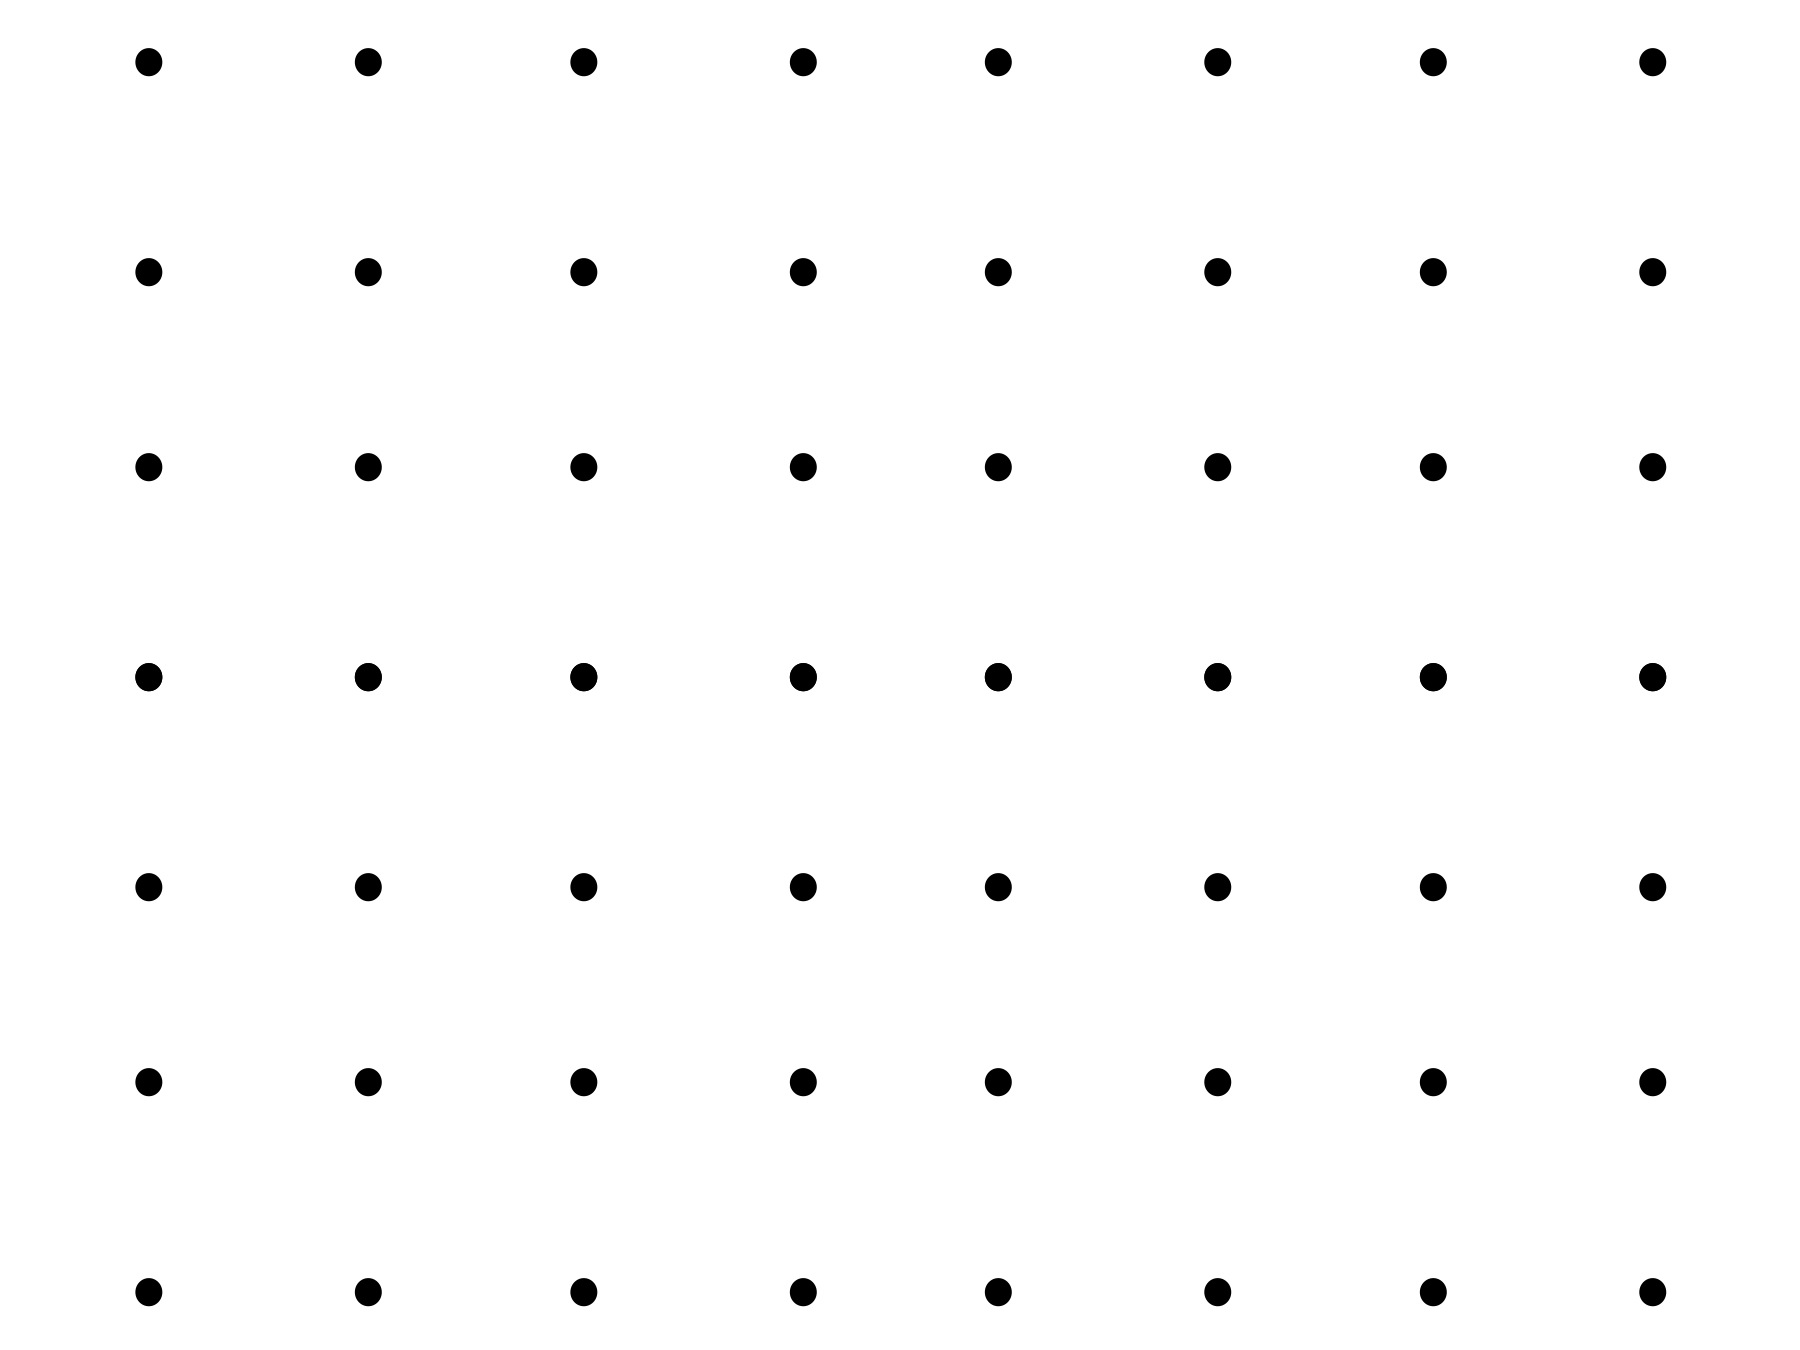
\includegraphics[scale=0.35]{gravitational-lensing/lensing3}
%	\end{center}
%\end{figure}

\section{Report Checklist}

Include the following in your lab report. See Appendix~\ref{cha:lab-report-format} for formatting details. Each item below is worth 10 points.

\begin{enumerate}
%	\item Explanation for higher incidence of lenses at higher redshift (Lab task 5)
	\item For each lens selected, the image of the lens, a table of name, $\theta_e$, redshift, and angular size distance $D_A$ (Steps 7--10)
	\item Calculation and final value for physical radii and masses (Step 11)
	\item Comparison to known maximum galaxy mass (Step 12)
	\item A 100--200 word reflection on group dynamics and feedback on the lab manual. Address the following topics: who did what in the lab, how did you work together, how group roles functioned, what successes and challenges in group functioning did you have, and what would you keep and change about the lab write-up?
\end{enumerate}